\documentclass[a4paper]{article}
\usepackage[spanish]{babel}
\usepackage[utf8]{inputenc}
\usepackage{graphicx}
\usepackage{biblatex}
\usepackage{enumerate}
\usepackage{csquotes}
\usepackage{braket}
\addbibresource{bibliografia.bib}

\title{Modos rotacionales y vibracionales en moléculas}
\author{José Soto García}
\begin{document}
\maketitle
\section{La molécula como un sólido rígido: hamiltoniano asociado a la rotación de la misma en torno a su centro de masas.}
Un sólido rígido se define como una colección de partículas, cuyas distancias relativas se mantienen fijas \cite{marion2013}. El momento de inercia $I_i$ de un sólido rígido con $n$ partículas sobre un eje $i$ se define como:
\begin{equation}
I_i= \sum_{j=1}^n=m_jr_j^2
\end{equation}
con $r_j$ la distancia desde la partícula de masa $m_j$ al eje $i$.

\subsection{El rotor rígido diatómico}
El rotor rígido de dos partículas consiste en dos masas $m_1$ y $m_2$ unidas a una barra sin masa con una distancia fija $d$. Dado que la distancia es fija, la energía potencial no varía con la rotación del rotor, luego $V=0$. \cite{levine1980} El momento de inercia de una molécula diatómica puede escribirse como:
\begin{equation}
I=\mu R^2
\end{equation}
Podemos determinar los niveles de energía de este sistema resolviendo la ecuación de Schrödinger. Suponiendo que el radio entre los dos átomos no varía, la ecuación de Schrödinger queda:
\begin{equation}
- \frac{\hbar^2}{2I}\left[\frac{1}{sin\theta}\frac{\partial}{\partial \theta}\left(sin\theta \frac{\partial}{\partial \theta} \right) + \frac{1}{sin^2\theta}\frac{\partial^2}{\partial \phi^2}\right]Y^m_l \left(\theta,\phi \right) = E_lY^m_l \left(\theta,\phi \right)
\end{equation}
Con
$$E_l= \frac{\hbar^2}{2I}l(l+1)$$
La energía está $2l+1$ veces degenerada debido a que para un $l$ fijo, distintos valores de $m$ tienen la misma energía.
\subsection{El rotor rígido poliatómico}
Se define el tensor de inercia $\tilde{I}$ como:
\begin{equation}
\tilde{I}=\left( \begin{array}{ccc}
\sum_{\alpha}m_{\alpha}\left(x^2_{\alpha,2}+x^2_{\alpha,3}\right) & -\sum_{\alpha}m_{\alpha}x_{\alpha,1}x_{\alpha,2} & -\sum_{\alpha}m_{\alpha}x_{\alpha,1}x_{\alpha,3} \\\\
-\sum_{\alpha}m_{\alpha}x_{\alpha,2}x_{\alpha,1} & \sum_{\alpha}m_{\alpha}\left(x^2_{\alpha,1}+x^2_{\alpha,3}\right) &-\sum_{\alpha}m_{\alpha}x_{\alpha,2}x_{\alpha,3} \\\\
-\sum_{\alpha}m_{\alpha}x_{\alpha,3}x_{\alpha,1} & -\sum_{\alpha}m_{\alpha}x_{\alpha,3}x_{\alpha,2} & \sum_{\alpha}m_{\alpha}\left(x^2_{\alpha,1}+x^2_{\alpha,2}\right) \end{array} \right)
\end{equation}
Clásicamente, la energía cinética rotacional del sistema se obtiene como:
\begin{equation}
T_{rot}=\frac{1}{2}\sum_{i,j}I_{i,j}\omega_i\omega_j
\end{equation}
Una clara simplificación se encuentra si diagonalizamos el tensor de inercia. Los vectores que diagonalizan la matriz de inercia son los denominados ejes principales de inercia. La energía cinética rotacional clásica del sistema queda por tanto \cite{marion2013}:
\begin{equation}
T_{rot}=\frac{1}{2}\left(I_a\omega^2_a + I_b\omega^2_b + I_c\omega^2_c\right) 
\end{equation}
con $I_a$, $I_b$, e $I_c$ los autovalores del momento de inercia.\\
Para formar el hamiltoniano del sistema, necesitamos la energía en función del momento angular $P$, con $P_i=I_i\omega_i$.
La energía cinética queda entonces como:
\begin{equation}
T_{rot}=\frac{P_a^2}{2I_a}+\frac{P_b^2}{2I_b}+\frac{P_c^2}{2I_c}
\end{equation}
El nuevo sistema de referencia $\left\lbrace a,b,c \right\rbrace$ se consigue mediante tres rotaciones  $\left\lbrace \theta,\phi,\chi \right\rbrace$ a través del centro de masas $O$. Son los llamados ángulos de Euler (figura \ref{euler}).
De la figura \ref{euler} podemos ver que:
\begin{equation}
\hat P_{\phi}=\frac{\partial}{\partial \phi},\,\ \hat P_{N}=\frac{\partial}{\partial N},\,\ \hat P_{\chi}=\frac{\partial}{\partial \chi}
\end{equation}

\begin{figure}
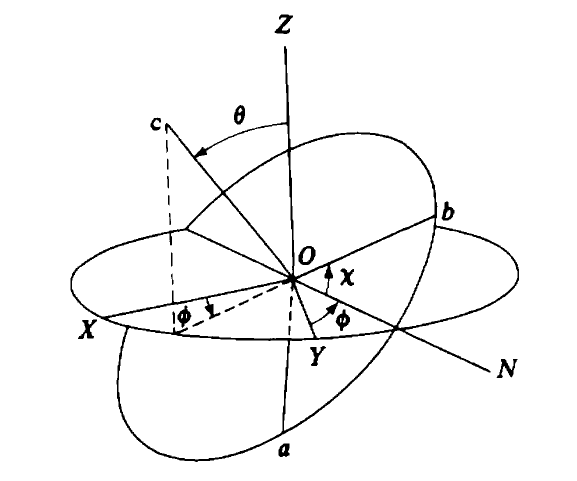
\includegraphics[width=0.8\textwidth]{Angulos_Euler.png}
\caption{EXPLICAR}
\label{euler}
\end{figure}

Teniendo en cuenta que 

$$ P_N=  P_a sin\chi + P_b cos\chi$$  
$$ P_Z= -P_a sin\theta cos\chi + P_b sin\theta sin\chi + P_c cos\theta $$

Obtenemos que:

\begin{equation}
\hat P_a = i\hbar \left[cos\chi csc\theta \frac{\partial}{\partial \phi} - cos\chi cot\theta \frac{\partial}{\partial \chi} - sin\chi \frac{\partial}{\partial \theta} \right]
\end{equation}
\begin{equation}
\hat P_b = i\hbar \left[-sin\chi csc\theta \frac{\partial}{\partial \phi} + sin\chi cot\theta \frac{\partial}{\partial \chi} - cos\chi \frac{\partial}{\partial \theta} \right]
\end{equation}
\begin{equation}
\hat P_c = -i\hbar \frac{\partial}{\partial\chi}
\end{equation}
O también:

\begin{equation}
\hat P_X = i\hbar \left[cos\phi cot\theta \frac{\partial}{\partial \phi} - cos\phi csc\theta \frac{\partial}{\partial \chi} + sin\phi \frac{\partial}{\partial \theta} \right]
\end{equation}
\begin{equation}
\hat P_Y = i\hbar \left[sin\phi cot\theta \frac{\partial}{\partial \phi} - sin\phi csc\theta \frac{\partial}{\partial \chi} - cos\phi \frac{\partial}{\partial \theta} \right]
\end{equation}
\begin{equation}
\hat P_Z = -i\hbar\frac{\partial}{\partial\phi} 
\end{equation}

Sabemos que el hamiltoniano rotacional es
\begin{equation}
\hat H_{rot}=\frac{\hat P_a^2}{2I_a}+\frac{\hat P_b^2}{2I_b}+\frac{\hat P_c^2}{2I_c}
\end{equation}
y el operador momento angular total es:
\begin{equation}
\hat P^2 = \hat P_a^2+  \hat P_b^2+  \hat P_c^2 = \hat P_X^2+  \hat P_Y^2+  \hat P_Z^2
\end{equation}
Una forma de obtener los autovalores de Energía sería sustituir los valores de P y resolver la ecuación de Schrödinger. Sin embargo, estos autovalores se pueden obtener mediante relaciones de conmutación.
Las relaciones de conmutación que necesitaremos son las siguientes:
\begin{equation}
\left[\hat P_i,\hat P_j\right]=-i\hbar\delta_{i,j}\hat P_k
\end{equation}
\begin{equation}
\left[\hat P_I,\hat P_J\right]=i\hbar\delta_{I,J}\hat P_K
\end{equation}
\begin{equation}
\left[\hat P^2,\hat P_j\right]=\left[\hat P^2,\hat P_J\right]=0
\end{equation}
\begin{equation}
\left[\hat P_J,\hat P_j\right]=0 \,,\ \forall_{J,j}
\end{equation}
con $J = \left\lbrace X,Y,Z \right\rbrace$ y $j= \left\lbrace a,b,c \right\rbrace$ \\
Con estas relaciones de conmutación es fácil comprobar que:
\begin{equation}
\left[H_{rot}, \hat P^2 \right] = 0
\end{equation}
\begin{equation}
\left[H_{rot}, \hat P_J \right] = 0
\end{equation}
\begin{equation}
\left[H_{rot}, \hat P_c \right] = i\hbar \left(\frac{1}{2I_a}-\frac{1}{2I_b}\right)\left(\hat{P_a}\hat{P_b}+\hat{P_b}\hat{P_a}\right)
\end{equation}
Puesto que $H_{rot}$ conmuta con $\hat{P^2}$ y con $\hat P_Z$,  se pueden elegir las autofunciones $\psi$ del hamiltoniano rotacional como autofunciones de ambos operadores. Además, como los operadores $\hat P_X, \,\ \hat P_Y \,\ y \,\ \hat P_Z$ cumplen las relaciones generales de conmutación del momento angular, obtenemos las siguientes relaciones:
\begin{equation}
\hat H\psi = E\psi
\end{equation}
\begin{equation}
\hat H\psi = J(J+1)\hbar \psi, \qquad J=0,1,2...
\end{equation}
\begin{equation}
\hat P_Z\psi = M\hbar\psi, \qquad M = 0,\pm 1,...,\pm J
\end{equation}
Los autovalores de energía dependerán de las simetrías de rotación que presente la molécula, estas son:\\
Rotor esférico $I_a=I_b=I_c= I$ \\
Rotor simétrico $I_a=I_b \neq I_c$ o $I_a\neq I_b=I_c$\\
Rotor asimétrico $I_a \neq I_b \neq I_c$\\
Tomaremos siempre los ejes principales de inercia de manera que $I_a\leq I_b\leq I_c$.
\section{Rotor rígido cuántico: Estados propios y autovalores.}
\subsection{El rotor esférico}
El rotor esférico se caracteriza porque los tres momentos principales de inercia son iguales: $$I_a=I_b=I_c= I$$
El hamiltoniano del sistema queda por tanto como:
\begin{equation}
\hat H = \frac{\hat P^2}{2I}
\end{equation}
La ecuación de Schödinger es:
\begin{equation}
\frac{1}{2I}\hat P^2 \psi = E\psi
\end{equation}
Resolviendo la ecuación obtenemos que:$$\frac{1}{2I}J(J+1)\hbar^2\psi=E\psi$$
\begin{equation}
E=\frac{J(J+1)\hbar^2}{2I}, \qquad J=0,1,2...
\end{equation}
En este caso, tenemos además que
\begin{equation}
\left[\hat H,\hat P_c \right]
\end{equation}
con $$\hat P_c \psi = K\hbar\psi, \qquad K = 0, \pm 1,..., \pm J$$
Luego la energía está $(2J+1)^2$ veces degenerada.
\subsection{El rotor simétrico}
El rotor simétrico se caracteriza porque dos de sus momentos principales de inercia son iguales $I_a=I_b\neq I_c$ (caso achatado) o $I_a\neq I_b=I_c$ (caso alargado). Realizaremos el desarrollo del caso $I_a=I_b\neq I_c$ y luego lo adaptaremos al segundo. 
El hamiltoniano del sistema es:
\begin{equation}
\hat H=\frac{\hat P_a^2+\hat P_b^2}{2I_b}+\frac{\hat P_c^2}{2I_c}=\frac{\hat P^2- \hat P_c^2}{2I_b}+\frac{\hat P_c^2}{2I_c}
\end{equation}
Como $\hat P_c$ conmuta con $\hat P^2$ y con $\hat P_c^2$, el hamiltoniano conmuta con $\hat P_c$, y las autofunciones del hamiltoniano se pueden elegir como autofunciones de $\hat P_c$.
Las energías se obtienen como: $$\left(\frac{\hat P^2- \hat P_c^2}{2I_b}+\frac{\hat P_c^2}{2I_c}\right)\psi=E\psi$$
 $$\left(\frac{\hbar^2J(J+1)- \hbar^2K^2}{2I_b}+\frac{\hbar^2K^2}{2I_c}\right)\psi=E\psi$$
 Luego:
 \begin{equation}
 E=\frac{\hbar^2J(J+1)}{2I_b}+\hbar^2K^2\left(\frac{1}{2I_c}-\frac{1}{2I_b}\right)
 \end{equation}
 Se definen las constantes rotacionales como:
 \begin{equation}
 A \equiv \frac{h}{8\pi^2I_a}\geq B\equiv \frac{h}{8\pi^2I_b}\geq C\equiv \frac{h}{8\pi^2I_c}
 \end{equation}
 Teniendo entonces que las energías son
 \begin{equation}
 E/h=BJ\left(J+1\right)+\left(C-B\right)K^2 \qquad (achatado)
 \end{equation}
 \begin{equation}
 E/h=BJ\left(J+1\right)+\left(A-B\right)K^2 \qquad (alargado)
 \end{equation}
La energía depende de $J$ y $K^2$. Hay una degeneración $(2J+1)$ asociada a $M$. Además, para $K\neq 0$ hay una degeneración doble debida a los valores de $\pm K$, luego para $K\neq 0$ la degeneración de la energía es $4J+2$.
\subsection{El rotor asimétrico}
En el rotor asimétrico $I_a\neq I_b\neq I_c$
En este caso, como $\left[\hat H,\hat P_c\right]\neq 0$ no podemos elegir las autofunciones de $\hat P_c$; además el hamiltoniano no es separable y necesitaremos otro método para resolver la ecuación de Schrödinger.\\
Podemos  encontrar los autovalores de $\hat H$ expandiendo las autofunciones desconocidas $\psi_i$ en términos de algún conjunto completo ortonormal conocido $\phi_i$ y resolviendo la ecuación de autovalores:
\begin{equation}
det \left[ \bra{\phi_n}\hat H\ket{\phi_m} - E_i\delta_{nm} \right]=0
\end{equation}
Un conjunto completo ortonormal que podemos usar son las autofunciones del rotor simétrico, ya que son funciones de las mismas coordenadas (los ángulos de Euler) y satisfacen las mismas condiciones de contorno:
\begin{equation}
\psi_i = \sum_{J'}\sum_{M'}\sum_{K'}c_{i,J'M'K'}\phi_{J'M'K'}
\end{equation}
Como $\psi_i$ es autofunción de $\hat P^2$ con autovalor $\hbar^2J(J+1)$ y de $\hat P_z$ con autovalor $\hbar M$ sólo necesitamos incluir fuciones $\phi_i$ con el mismo valor de $J$ y $M$ que $\psi_i$. La suma infinita sobre $J'$, $M'$ y $K'$ se reduce ahora a una suma finita sobre los $2J+1$ posibles valores de $K'$
\begin{equation}
\psi_i = \sum_{K'=-J}^Jc_{i,JMK'}\phi_{JMK'}
\end{equation}
Luego, la ecuación de autovalores queda:
\begin{equation}
det\left(H_{K'K''}-E_i\delta_{K'K''}\right)=0
\end{equation}
con
\begin{equation}
H_{K'K''}\equiv\int\phi^*_{JMK'}\hat H\phi_{JMK''}d\tau
\end{equation}
Cuyo resultado es calculable con los datos que tenemos y vale:
$$
H_{K'K''}=\delta_{K''K'}\frac{1}{2}h\left[\left(2C-A-B\right)\left(K'\right)^2+\left(A+B\right)J\left(J+1\right)\right]$$$$+\delta_{K''K'+2}\frac{1}{4}h\left(B-A\right)\left[J\left(J+1\right)-K'\left(K'+1\right)\right]^\frac{1}{2}$$$$\cdot\left[J\left(J+1\right)-\left(K'+1\right)\left(K'+2\right)\right]^\frac{1}{2}$$$$+\delta_{K''K'-2}\frac{1}{4}h\left(B-A\right)\left[J\left(J+1\right)-K'\left(K'-1\right)\right]^\frac{1}{2}$$
\begin{equation}
\cdot\left[J\left(J+1\right)-\left(K'-1\right)\left(K'-2\right)\right]^\frac{1}{2}
\end{equation}
Siendo
$$
A \equiv \frac{h}{8\pi^2I_a}\geq B\equiv \frac{h}{8\pi^2I_b}\geq C\equiv \frac{h}{8\pi^2I_c}
$$
Podemos ver que los autovalores del hamiltoniano no dependen de $M$, por tanto, la degeneración de la energía será $2J+1$, correspondientes a los posibles valores de $M$ para un $J$ dado.
Cada función de onda del rotor asimétrico $\psi_i$ es una combinación lineal de las $2J+1$ funciones de onda de del rotor simétrico con los mismos valores de $J$ y $M$ que $\psi_i$.

\section{Estructura del espectro rotacional.}
\newpage
\printbibliography
\end{document}

